\begin{longtable} { | c | p{12cm} | c | } 
\hline
	ID 	&	Issues	&		 Es. hours \\\hline
	42	&	Add preview Button	&	1 hours	\\\hline
\caption{Issue ID 42}
\label{tab:spr4_previewButton}
\end{longtable}

Guardians stated that they needed a way to quickly view a sequence. This would require returning to overview, pressing the log out button, choosing a child with the sequence and then opening it. For this reason it was decided to implement a preview button in SequenceActivity. The implemented functionality prompts the guardian that the sequence will be saved and then continues to display the sequence in Sequenceviewer. The reasoning behind saving the sequence is to make it compatible with a call to Sequenceviewer. Sequenceviewer is launched with an \ct{intent} containing the ID of the sequence to display. This is something given through the database, for which reason it must be saved. It would not be able to pass Sequenceviewer the sequence directly through an \ct{intent}, as only simple types are supported. Thus, the easy solution was to ask the user to save the sequence first. This behavior can be seen in \ref{fig:savebeforepreview}.

\begin{figure}[H]
	\centering
	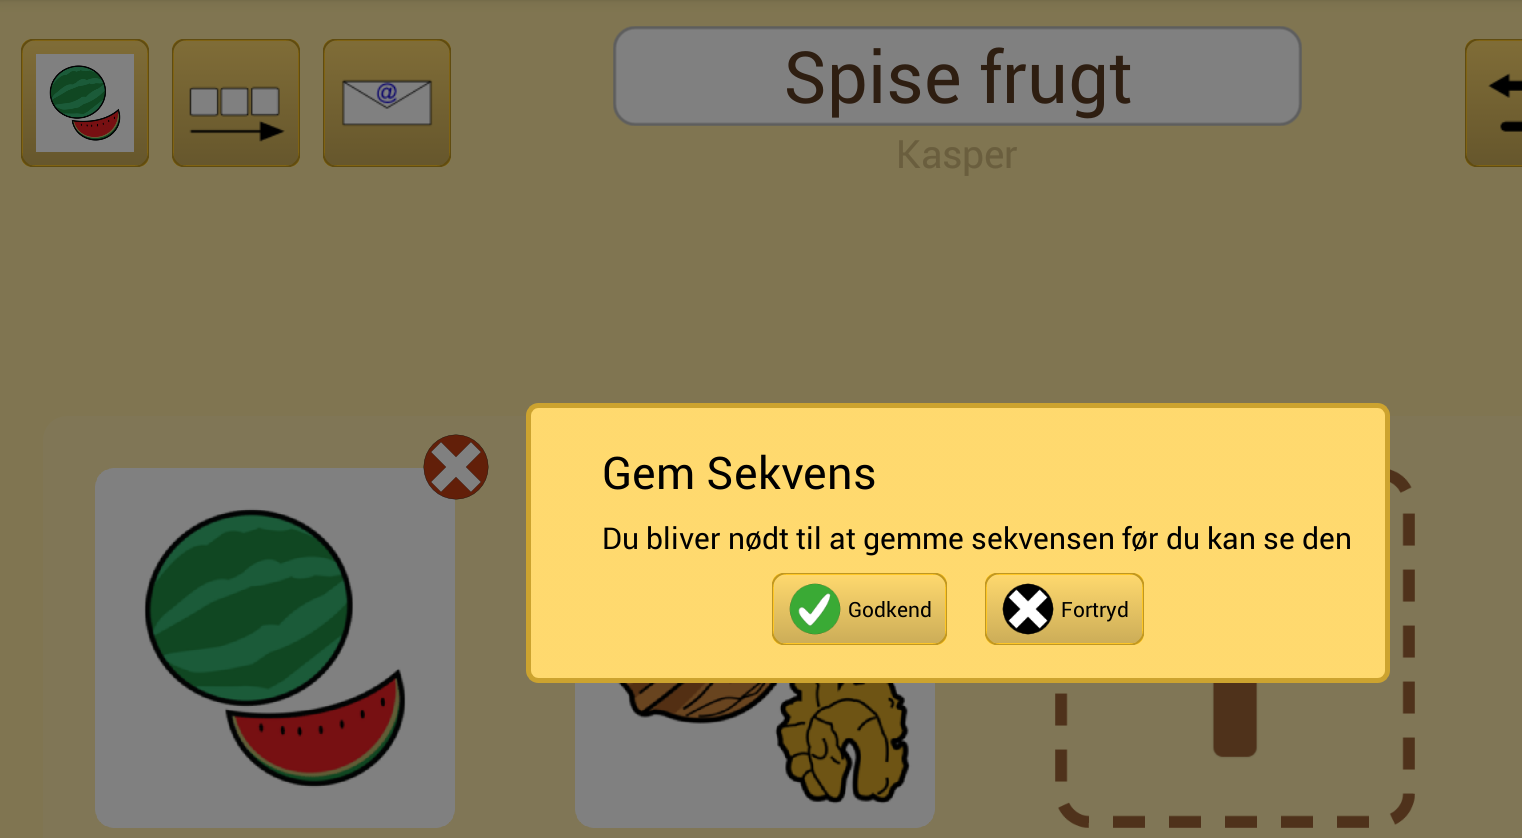
\includegraphics[width=0.95\textwidth]{Pics/Sprint4/savebeforepreview.png}
	\caption{Prompting the user to save sequence before displaying it}
	\label{fig:savebeforepreview}
\end{figure}